\documentclass[border=5mm]{standalone}
\usepackage{pgfplots}
\pgfplotsset{compat=1.10}
\begin{document}
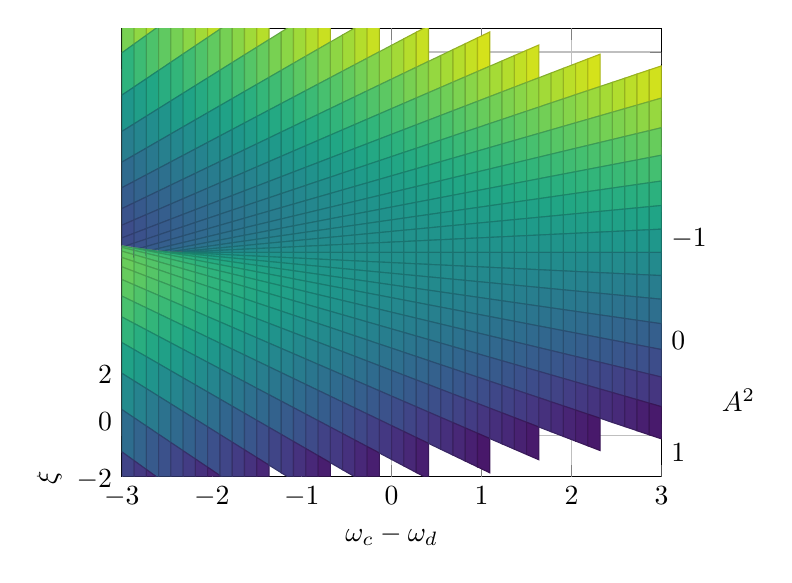
\begin{tikzpicture}
\begin{axis}[
          anchor=origin,
          rotate around={0:(current axis.origin)},
          y domain=-3:3,
          domain=-2:2,zmin=-3,zmax=3,
          restrict z to domain=-5:5,
          samples=45,
          view={90}{65},
          mesh/interior colormap name=viridis,
          colormap/blackwhite,
          xlabel=$A^2$,ylabel=$\omega_c-\omega_d$,zlabel=$\xi$,grid=both
         ]
\addplot3[surf] {-4*x^3 - 2*y*x};
\end{axis}
\end{tikzpicture}
\end{document}
